%%%%%%%%%%%%%%%%%%%%%%%%%%%%%%%%%%%%%%%%%%%%%%%%%%%%%%%%%%%%%%%%%%%
%TO AVOID FORMATTING ISSUES, COMPILE THIS ONLY AT WWW.OVERLEAF.COM%
%%%%%%%%%%%%%%%%%%%%%%%%%%%%%%%%%%%%%%%%%%%%%%%%%%%%%%%%%%%%%%%%%%%
%AUTHOR: 
%CLASS:  
%%%%%%%%%%%%%%%%%%%%%%%%%%%%%%%%%%%%%%%%%%%%%%%%%%%%%%%%%%%%%%%%%%%
\documentclass[a4paper,12pt]{article}
\usepackage{graphicx}
\newenvironment{codeblock}{\fontfamily{pcr}\selectfont}{\par}

\title{
	\normalfont \normalsize 
	\textsc{Pimpri Chinchwad College of Engineering \\ 
		Computer Laboratory - III} \\
	[10pt] 
	\rule{\linewidth}{0.5pt} \\[6pt] 
	\huge Assignment No - 5 \\
	\rule{\linewidth}{2pt}  \\[10pt]
}
\author{}
\date{\normalsize}


\begin{document}
\maketitle

%%%%%%%%%%%%%%%%%%%%%%%
% FOR A NUMBERED LIST
% \begin{enumerate}
% \item Your_Item
% \end{enumerate}
%%%%%%%%%%%%%%%%%%%%%%%
% FOR A BULLETED LIST
% \begin{itemize}
% \item Your_Item
% \end{itemize}
%%%%%%%%%%%%%%%%%%%%%%%
% TO IMPORT AN IMAGE
% \includegraphics[width=\textwidth]{name_of_file}
% \textwidth makes the picture the width of the paragraphs
%%%%%%%%%%%%%%%%%%%%%%%%%%%%%%
% TO CREATE A FIGURE WITH A NUMBER AND CAPTION
% \begin{figure}
% \includegraphics[width=\textwidth]{image}
% \caption{Your Caption Goes Here}
% \label{your_label}
% \end{figure}
% REFER TO YOUR FIGURE LATER WITH
% \ref{your_label}
% LABELS NEED TO BE ONE WORD
%%%%%%%%%%%%%%%%%%%%%%%%%%%%%
% TO ADD CODE
% \begin{codeblock}
% Some code in "courier" font
%\end{codeblock}
%%%%%%%%%%%%%%%%%%%%%%%%%%%%%
\section{Aim}
	\paragraph{} Write a Python/ Java/c++ program to validate the parameter tuple \{p,q,g\} for the security of the DSA. Use Miller-Rabin primality test determine whether a given number is composite or probably prime.
	
\section{Objective}
	\begin{itemize}
	\item To Understand how to do Primality Test.
	\item To learn Miller Rabin Algorithm for Primality Test.
	\end{itemize}
	
\section{Software Requirements}
	\begin{itemize}
		\item	Windows
		\item	Java
	\end{itemize}
	
\section{Mathematical Model}
\paragraph{} 
S 	= {s, e, x, y, Fme, DD, NDD}  											\\\\
S   =   Initial State  														\\
E 	=   End State  															\\
X	= Input Value															\\
X=\{x1\} 																\\
where,  x1= p 												\\
 																\\
Y	= Output																\\
Y=\{y1\}																	\\
y1=\{True/False\}									\\
Fme 	= 	Main function 													\\
Fme=\{f1\}\\f1="Miller Rabin algorithm is used to check primality of a given number".		\\
													\\											\\
DD 	= 	Deterministic data \{Number p\}					\\
NDD	= 	Non Deterministic Data \{Primality \}							\\
		
		
	
\section{Theory}
		\paragraph{} 
	\subsection{Primality Test}
		    

	\begin{itemize}
	    \item Given an integer n, how can we tell if n is prime? The most obvious way is to look for factors of n, but no efficient factoring algorithm is known.
	    \item From now let us assume n is odd, since deciding the primality of an even number is trivial.
	    \item By Fermat’s Theorem, if \textbf{n} is prime, then for any \textbf{a} we have $a^{n-1}=1(mod n)$. This suggests the Fermat test for a prime: pick a random a\\epsilon\{1,...,n-1\} and see if  $a^{n-1}=1(mod n)$. If not, then n must be composite.
	    
	    
	  
	\end{itemize}
	
	\subsection{The Miller Rabin Test}
	\begin{itemize}
	    \item	A primality test that provides an efficient probabilistic algorithm for determining if a given number is prime. It is based on the properties of strong pseudoprimes.

        \item The algorithm proceeds as follows. Given an odd integer n, let $n=2^{r}s+1$ with s odd. Then choose a random integer a with $1<=a<=n-1$. If $a^{s}=1 (mod n)$ or $a^{(2^{j}s)}=-1 (mod n)$ for some $0<=j<=r-1$, then n passes the test. A prime will pass the test for all a.

\item The test is very fast and requires no more than (1+o(1))logn multiplications (mod n), where log is the logarithm base 2. Unfortunately, a number which passes the test is not necessarily prime. Monier (1980) and Rabin (1980) have shown that a composite number passes the test for at most 1/4 of the possible bases a. If N multiple independent tests are performed on a composite number, then the probability that it passes each test is $(1/4)^{N}$or less.
\item 
However, if the smallest composite number that passes a particular set of tests is known ahead of time, then that set of tests constitutes a primality proof for all smaller numbers. The sequence of smallest odd numbers passing a multiple Rabin-Miller test using the first k primes for k=1, 2, ... is given by 2047, 1373653, 25326001, 3215031751, 2152302898747, 3474749660383, 341550071728321, 341550071728321, ... (OEIS A014233; Jaeschke 1993). Therefore, multiple Rabin tests using the first 7 primes (using 8 gives no improvement) are valid for every number up to $3.4*10^{(14)}$.
\item 
The Wolfram Language implements the multiple Rabin-Miller test in bases 2 and 3 combined with a Lucas pseudoprime test as the primality test used by the function Prime Q[n]. As of 1997, this procedure is known to be correct only for all $n<10^{(16)}$, but no counterexamples are known and if any exist, they are expected to occur with extremely small probability (i.e., much less than the probability of a hardware error on a computer performing the test)

	\end{itemize}	
\section{Algorithm}
	
  \begin{verbatim}
Input: n > 2, an odd integer to be tested for primality;
       k, a parameter that determines the accuracy of the test
Output: composite if n is composite, otherwise probably prime
write n - 1 as 2s.d with d odd by factoring powers of 2 from n - 1
LOOP: repeat k times: 
    pick a randomly in the range [2, n - 1] 
   x ← ad mod n 
   if x = 1 or x = n - 1 then do next LOOP 
   for r = 1 .. s - 1 
      x ← x2 mod n 
      if x = 1 then return composite 
      if x = n - 1 then do next LOOP 
   return composite 
return probably prime

  \end{verbatim}
  \subsection{Parameter Generation}
  The first part of the DSA algorithm is the public key and private key generation, which can be described as: 
    \begin{codeblock}
    \begin{enumerate}
        \item Choose a prime number q, which is called the prime divisor.
        \item Choose another primer number p, such that p-1 mod q = 0. p is called the prime modulus.
        \item Choose an integer g, such that 1 < g < p, $g^{q}$ mod p = 1 and g = $h^{(p–1)/q)} mod p$. q is also called g's multiplicative order modulo p.
        \item Choose an integer, such that 0 < x < q.
    Compute y as $g^{x}$ mod p.
    	\item Package the public key as {p,q,g,y}.
    Package the private key as {p,q,g,x}.
	\end{enumerate}
    \end{codeblock}
    
  
\section{Example}
	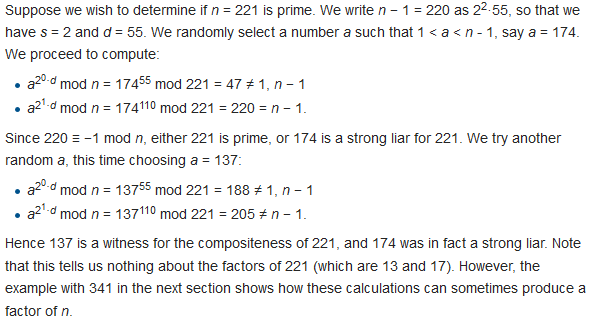
\includegraphics[width=\textwidth]{rabin_example}

\section{Testing}
\subsection{Positive Testing}

   \textbf{ Input}: Prime Number.\\
    \textbf{Output}:Number is Composite.\\
    
    
\subsection{Negative Testing}
   \textbf{ Input}:Non Prime Number.\\
   \textbf{ Output}:Number is Inconclusive.\\
    
    
\section{Conclusion}
	\paragraph{} Thus, We have studied and implemented miller-rabin algorithm to perform primality test.
\vspace{20px}
\begin{center}
	\begin{tabular}
		{|c|c|c|c|}\hline
		{\bf Roll No.}		&{\bf Name of Student}		&{\bf Date of Performance}  				&{\bf Date of Submission}  \\ \hline
		{302}	&	{Abhinav Bakshi}& {18/02/2016}		&  {10/03/2016}\\ \hline
	\end{tabular}\\ 
\end{center}

\section{Plagarism Report}
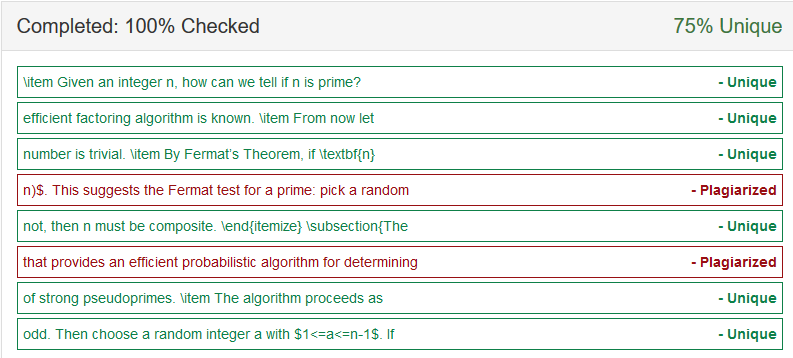
\includegraphics[width=\textwidth]{rmpl}
\section{Output}
\begin{verbatim}
---------------------------------------------
Miller Rabin output

Enter Number to test : 
71
Inconclusive


Generation
Parameters : 
p : 2983
q : 71
g : 425

--------------------------------------------
\end{verbatim}

\end{document}
 

 
